%
% file: main.tex
% date: 2003-01-10
%   by: GDB
% desc: Android Paper
%

\documentclass[11pt]{article}
\usepackage{times}
\usepackage{vmargin}
\usepackage{epsfig}
\usepackage{url}
\usepackage{verbatim}
\usepackage{myfancybox}
\usepackage{graphics}
%\usepackage{vfile}
\usepackage{subfigure}

% use custom frame environments
\input{frames.tex}

\def\inotify{iNotify}

% Some useful macros

% Multiline comments
\long\def\com#1{}

% Document configuration

% Margins
\setpapersize{USletter}
%\setmarginsrb{left}{top}{right}{bottom}
%\setmarginsrb{1.0in}{1.0in}{1.0in}{1.0in}{0pt}{0mm}{0.25in}{7mm}
\setmarginsrb{1.0in}{1.0in}{1.0in}{1.0in}{0pt}{0mm}{0.25in}{7mm}

\begin{document}

\centerline{\LARGE Sync ......}
\vspace{0.05in}
\centerline{\LARGE for android}
\vspace{0.20in}
\centerline{\large Peter Burns
            \hspace{0.25in} Lihuan(Riku) Xie
            \hspace{0.25in} Peter S. Pacheco}
\vspace{0.20in}
\centerline{Department of Computer Science}
\centerline{University of San Francisco}
\centerline{2130 Fulton Street, San Francisco, CA 94117-1080}
\centerline{\{rictic, rikutse, xeno.zhang\}@gmail.com}
%\vspace{0.20in}
%\centerline{{\bf Full Paper}}
\vspace{0.60in}


\begin{abstract}
	In this paper we present \teledroid, a synchronization service for android to aid the need of making use of cloud 
computing facilities to get more powerful computational ability and faster execution with longer battery life. \\

\teledroid\ use a SSH connection between server and mobile device to communicate and determine the files to be transfered. 
A simple SCP implementation was included in \teledroid\ to conduct the task of transfer files. \teledroid\ employes the 
operating system feature of monitoring file changes in file systems, which in Linux is inotify, to trace file system 
changes. The changes from both local and remote will then be analyzed and generate the file changes list and syntonization 
 action list. We use several techniques to prevent ping-pong syntonization, including temporary unregistering file from inotify when transfer file and touching the file modification time after transfer. \\

We conduct experiments in the paper to find out whether \verb+inotify+ could provide performance advantages over 
traditional file scan method.

\end{abstract}

% do the keywords
%\begin{keywords}
%\noindent
%Keywords: {\bf Parallel I/O, Linux, Multiprocessors, Threads}

%\end{keywords}

\pagebreak

\section{Introduction}
\label{sec:Introduction}

You could use ~\cite{Google:2008} to add reference listed in android.bib 
which could be easily generated by reference management applications.


The rest of this paper is organized as follows.
Section~\ref{sec:Motivation} describes the motivation of \teledroid\ project.
Section~\ref{sec:Architecture} describes the architecture of \teledroid\ project.
Section~\ref{sec:Implementation} provides the implementation details.
Section~\ref{sec:Synchronization} emphasizes the synchronization mechanism of \teledroid.
In section~\ref{sec:Performance}, we will conduct series of experiments to evaluate the performance of \teledroid, and compare the performance differences between syncing modes. 
We will discuss related work in section~\ref{sec:Related}. 
In section~\ref{sec:Conclusions} we conclude and present our possible future work.

Use ref to auto locate the section number.

{\bf Acknowledgments}  Here's the acknowledgments.
\section{Motivation}
\label{sec:Motivation}
% Peter
\section{Architecture}
\label{sec:Architecture}
Regarding the design of \teledroid\ Application, there are three main components in the architecture, as in 
Figure~\ref{fig:architecture}. Initially, we implement a file browser activity as our main activity in \teledroid\ app. 
Users is able to view all the files in Android file system. Besides, the file browser can open the files of at lease 
audio, plain text, and image format. We use this file browser for testing purpose. Next, a long-time running and local 
service can be started from the menu on the file browser activity. The service will stay connecting with server even when 
\teledroid\ is no longer visible. This background service serves with the functionalities of monitoring, scanning, and 
syncing files with remote server. At last, note that two sorts of threads will be invoked by the background service. 
There are \verb+FileMonitorThread+, and \verb+ScanFilesThread+. We prefer to implement threads rather than all the 
functions within one process because we could like to decouple each functionality so as to relieve the synchronization 
issue. 

\begin{figure}[htp]
\centering
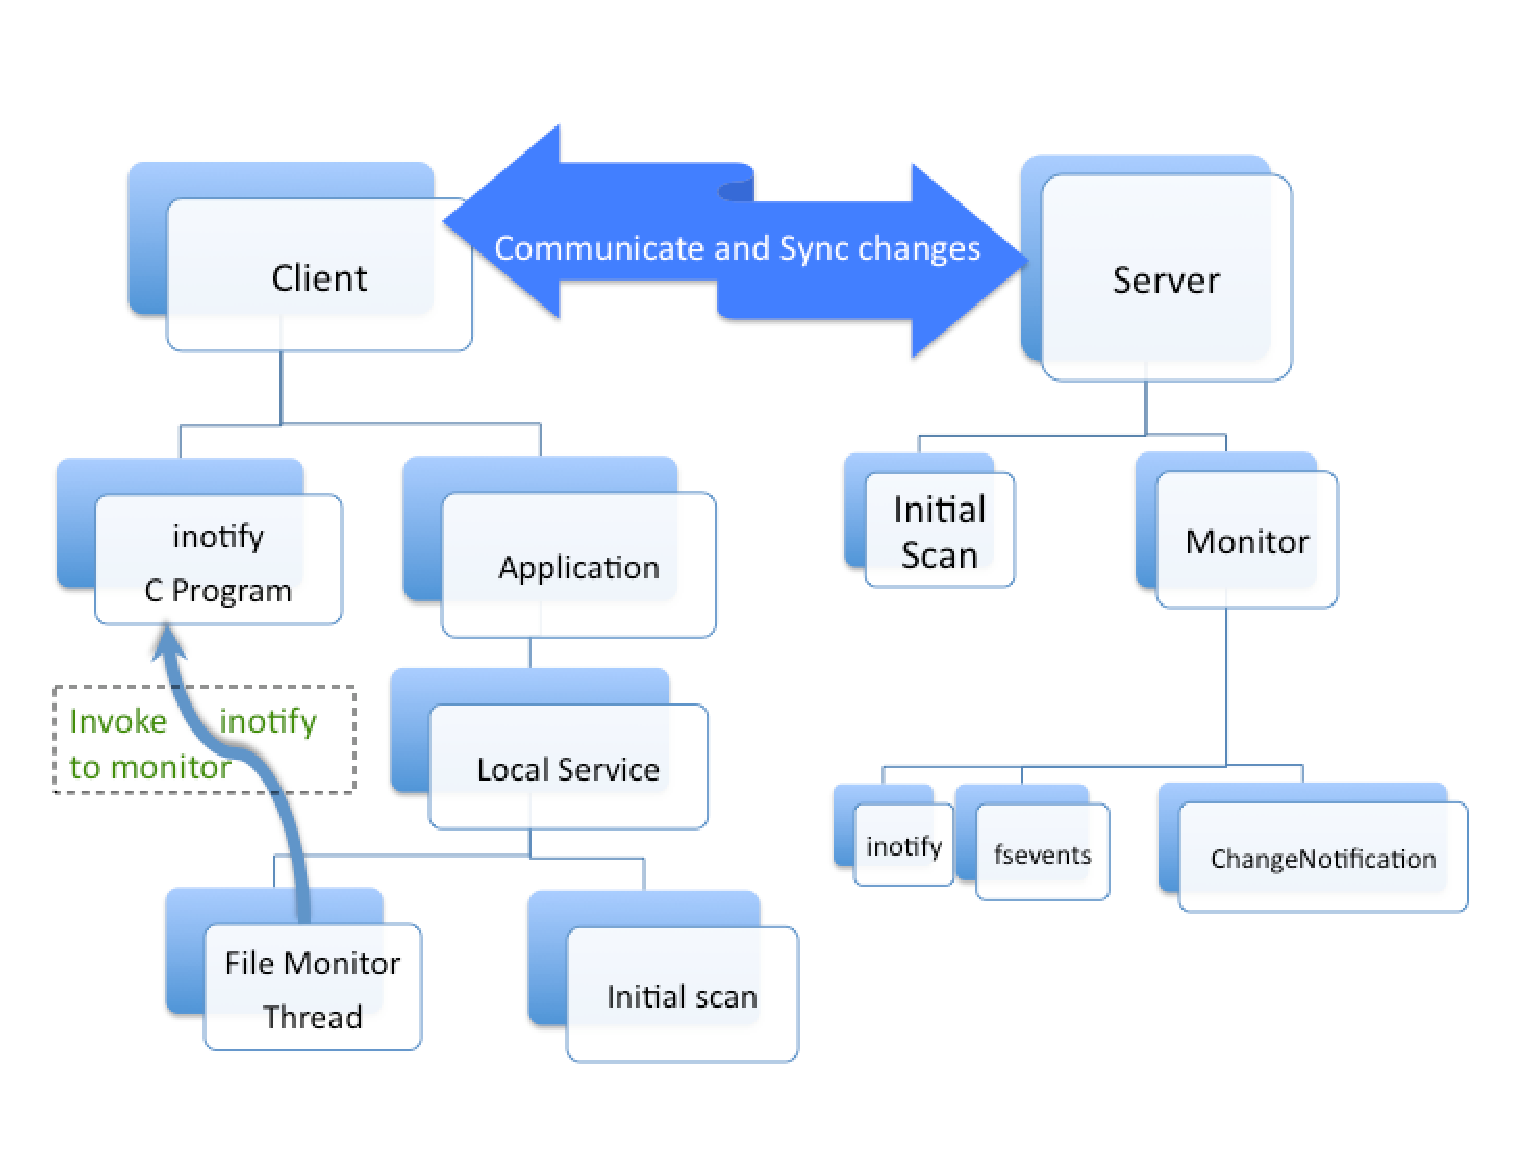
\includegraphics[scale=0.5]{architecture}
\caption{\teledroid\ Architecture}\label{fig:architecture}
\end{figure}

\section{Implementation}
\label{sec:Implementation}
\subsection{Client Server Communication}
Our implementations of the the communication and file transfer are based on JSch. JSch is a pure java open source SSH library. We will establishing internet connection with remote server when application starts, and keep the connection open. As our background service will communicate with remote server from time to time, and transfer back and forth. 

JSch library provides the ability to open different channels simultaneously using only one session, so that we could avoid 
wasting time and resource establishing the connection. We implements a class \verb+Connection+ and put in all the 
connection related functions, including open shell channel and transfer file over SCP. We implement function to open 
a shell for executing command on server, scan remote file information and comparing the changes lists from local and server 
using JSON. We also implement two functions \verb+SCPTo()+ and \verb+SCPFrom()+ follows the SCP protocol for transferring files with time 
difference to keep both side synchronized. As we could have several concurrent ongoing channels connected with server at 
the same time, we could have shell channels to persistently communicate with remote server, and meanwhile still be able 
to transfer files. By getting output stream from channel, we could receive output data from the shell of remote server. 
Similarly, \teledroid\ could execute command on server by writing a input stream to the Shell channel. 

We use FIFO algorithm during the scan of the filesystem, either looking for changes or registering files. A root directory is pushed into a stack at the initial time. Then, with popping out the root directory, we scan all the files in the root directory. If the files are also directory, we push them back to stack. If not, the file name with absolute path and the modified time of that file will be stored in a list. Recursively, we will retrieve the modified time of all the files in root directory in a list or register all the files in the root directory into notify. 

By executing command on server, we can get the same kind of list from server or register server into inotify and retrieve file change list. Those two lists will be converted to JSon object, which is a collection of name/value pairs with more powerful supports. \teledroid\ will then compare these two JSon objects. If the difference of the modified time of the same file is bigger than one second, the younger copy of file will be synced and replaced the old one on the other side with changing the modified time as the same as the younger one. By this method, we are able to avoid the synchronization issue that syncing back and forth the file because of the modified time of the new files after replacement. More details are on Synchronization section of this paper.

\subsection{File Change Notification}
Our application design requires a file change notification system, which should allow applications to request 
the monitoring of a set of files against a list of events. As the nature of running on mobile device, it should 
only require very little system resource and be able to be easily invoked in user space. 

Our implementation of filesystem monitor is based on inotify. inotify is an inode-based file notification system 
that does not require a file ever be opened in order to watch it. It is designed with an interface that user space 
application could easily accessed through system calls. Also, inotify communicates with applications via a single 
file descriptor instead of signals providing simple and fast invocation.

For Linux, inotify was included in the mainline kernel from release 2.6.13 (June 18, 2005)\cite{Love:2005p1294}. We 
checked the default compilation option for Android, the support for inotify was not removed. So we wrote a piece of 
C program to make sure the inotify in emulator. The result was very encouraging. And we also found that in Android, 
the toolbox have implements a simple notify program using the inofity system call. However, the attempt of using the 
system provided notify was unsuccessful. When the notify program was running, our program can get nothing back from 
its stdout. After excluding the possibility of permission issue, we located the problem. Android notify program will 
not flush the output stream after writing the result, so our application will block when reading from notify output 
stream. 

In our first release, we implement our own notify program, cross-compiled and pushed into Android environment. This 
program simply implements the functionality of the original google version notify program but will flush the output 
stream every time it finishes writing. The problem with this implementation is obvious. We have to create an extra process 
and stream with it to communicate. And also, in this way we cannot register and unregister for single files freely. 
We could only monitor a directory at a time, or we have to create multiple processes of notify program, which will surely 
affect the performance. 

In the final release, we use Android JNI Library to invoke the inotify system calls. JNI is not officially supported by 
google, so there's no documentation for it. We implement a static class Notify as the interface to our notify library. 
In the \verb+libnotify+, we use \verb+initNotify()+ to initialize inotify and get the file descriptor. We implement two 
method \verb+registerFile()+ and \verb+unregisterFile()+ for registering file to be monitored and release the monitor. 
We also implements \verb+hasNext()+, \verb+nextEvent()+ and \verb+eventMask()+ to get the event information. And if the 
event is with a subfile of directory, we use \verb+newFile()+ to get the sub file information. We cross-compiled the 
library and put generated \verb+libnotify.so+ into the lib directory for our application: 
\verb+data/data/net.solarvistas.android/lib/+, so that in java static class Notify constructor, we could use 
\verb+System.loadLibrary(``notify'')+ to load the library. 

We met a problem when compile the C library, the JavaVM passed into \verb+JNI_Onload()+ cannot be correctly recognized 
as struct. So we ignored the JNI\_VERSION check and implements native method \verb+registerNativeMethod()+ to register 
the JNI native methods. We also include \verb+<utils/Log.h>+ so that we could retrieve these information from Android 
ddms logcat.

\subsection{Server Side Script}
The server-side portion of the project was broken into two parts, corresponding to the two phases of interaction with the server. Initially we construct a mapping of filename to modified time for each file in the portion of the filesystem we're synchronizing by doing a simple walk. This is inefficient in both time and space, but unavoidable, as monitoring for changes on both server and client side is only useful if they're initially synchronized.

After the client receives and processes the mapping of the entire directory, it launches a process that watches for changes. Two approaches were implemented here, pull and push. The pull-sync program gathers changes silently, sending them all in a batch on demand, while push-sync sends each change immediately, as it happens.

This work was implemented in the Factor programming language.  Factor is a high level, stack based language with an efficient optimizing compiler.  While a very interesting language in its own right, it is still a young language.  It was chosen for \teledroid purely for pragmatic reasons, however.  Due in part to its excellent foreign function interface, it is the only known environment with a cross-platform API for filesystem monitoring, with bindings for Linux's inotify, Mac OSX's fsevents, and a family of functions in the win32 API.

JSON was used as a serialization format as its impedance mismatch to our data – mostly maps from strings to long integers – was minimal.  JSON also had the advantage of actually being easy for humans to read while debugging.



\subsection{Synchronization}
Synchronization is one of the significant element in a distributed system. The issue in our \teledroid\ application is that the file after replacement will generate a new modified time, which is the current time and later than the file on the other side. Thus, file on the other side will be replaced and also generate a newer modified time. Again and again, that file will be transferred back and forth even without any content modification. This is the result of applying the modified time as a key to the file comparison. We could employ checksum in our system, this might relieve the issue a little. However, the checksum approach has a hard time to cope with distinguishing the new and the deleted files. So now, our working version only support comparison with the modified time. Our solution so far is that the new generated file will not has the current time as the modified time. Instead, it will be assigned with the modified time of that modified file on the other side. In this way, \teledroid\ will prevent from transferring files back and forth and become more efficient.

\subsection{Extra Parts}
(Riku)

\section{Synchronization}
\label{sec:Synchronization}
Synchronization is one of the significant element in a distributed system. The issue in our Teledroid application is that the file after replacement will generate a new modified time which is the current time.


\section{Performance Evaluation}
\label{sec:Performance}

We conducted our tests in two different mode: scan mode, and monitor mode. In scan mode, the relevant portion of the filesystem is scanned and a tree is built of modification times, both locally and on the server.  The server then sends this information down to the local device, where they are compared to determine what needs to be synchronized. In monitor mode, we use filesystem monitors to watch for changed files on both server and client side, so the only files that are considered for synchronization are those which changed. 

%more info is needed here on how the tests were actually carried out

\subsection{Testing Plan}
In our experiments, we ran the \teledroid application on the background. In turn, we updated multiple files, totaling 1MB in size, on both the local device and the server side three times. In the experiment, we captured CPU and memory usage every 10 seconds. After \teledroid completed one round of file transfers, we recorded the time spent. The experiments were done in both scan mode and monitor mode.
			
\subsection{Hardware Configuration}
Our test device is an Android Dev Phone 1. It has a 528MHZ Qualcomm 7210 processor and 192 MB RAM. It features a touch screen and a trackball for navigation, and provides QWERTY slider keyboard for input. Wi-Fi, GPS, and Bluetooth v2.0 are also present. It also supports 3G WCDMA in 1700/2100 MHz and Quad-band GSM in 850/900/1800/1900 MHz. Note that the Android Dev Phone 1 includes 1GB MicroSC card as an external storage device. It can be replaced with a card of up to 16GB. Concerning the network environment, our tests utilized the University of San Francisco's internet connection, accessed through 802.11g.

\subsection{Results}
The results of our CPU usage tests are shown in Figure~\ref{fig:cpu}. However they were not as we expected. Monitor mode didn't gain any significant advantage over scan mode here. However, synchronization finished faster than in scan mode, so overall cpu usage should be lower than our tests indicate.

\begin{center}
  \begin{tabular}{ | l || c | c | c | c | c | c | c | c | c | c | }
    \hline
CPU Usage& 1  & 2	 & 3 	& 4 	& 5 	& 6 	& 7 	& 8 	& 9 	& 10	 	\\ \hline\hline
Scan	& 2\% & 64\% & 92\%	& 94\% 	& 78\% 	& 4\%	& 80\%	& 91\%	& 92\%	& 16\% 	  	\\ \hline
Monitor	& 0\% & 86\% & 55\%	& 85\% 	& 86\% 	& 42\%	& 24\%	& 4\%	& 75\%	& 45\% 		\\ \hline\hline

CPU Usage& 11 & 12	 & 13	& 14	& 15	& 16 	& 17 	& 18 	& 19 	& 20 		\\ \hline\hline
Scan	& 4\% & 8\%	 & 92\%	& 88\% 	& 0\% 	& \%	& \%	& \%	& \%	& \%  		\\ \hline
Monitor	&75\% & 91\% & 93\%	& 88\%	& 34\% 	& \%	& \%	& \%	& \%	& \%  		\\ \hline\hline

CPU Usage& 21 & 22	 & 23	& 24	& 25	& 26 	& 27 	& 28 	& 29 	& 30 		\\ \hline\hline
Scan	& \% & \%	 & \%	& \% 	& \% 	& \%	& \%	& \%	& \%	& \%  		\\ \hline
Monitor	& \% & \% 	 & \%	& \%	& \% 	& \%	& \%	& \%	& \%	& \%  		\\ \hline\hline
  \end{tabular}
\end{center}

%	& \% 	& \%	& \%	& \%	& \% 	& \%

%92\%	88\%
%62\%	72\%
%93\%	41\%
%5\%	92\%
%4\%	77\%
%92\%	92\%
%70\%	7\%
%84\%	4\%
%0\%	
%2\%	
%93\%	
%76\%	
%2\%	
%1\%

\begin{figure}%[htp]
\centering
\subfigure[CPU Usage in Monitor Mode]{\label{fig:cpu-monitor}
    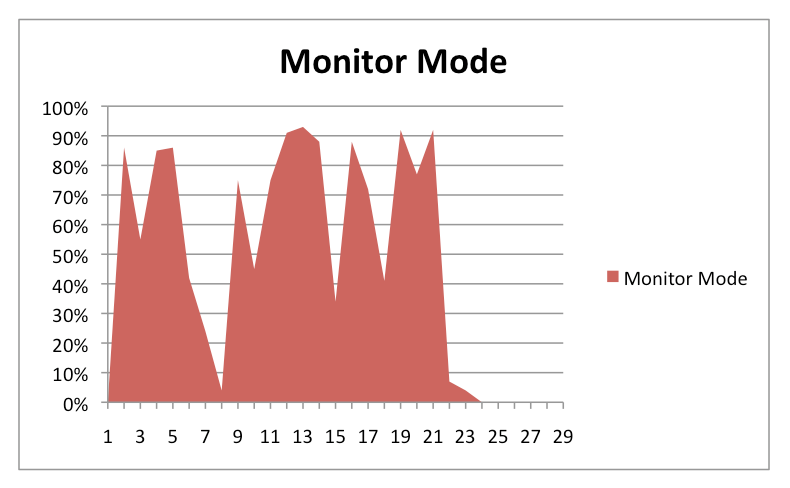
\includegraphics[scale=0.5]{cpu_monitor}}
\subfigure[CPU Usage in Scan Mode]{\label{fig:cpu-scan}
	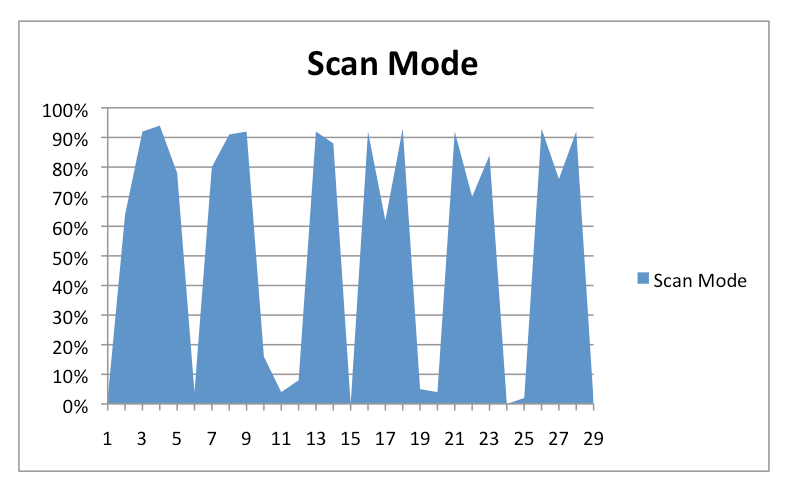
\includegraphics[scale=0.5]{cpu_scan}}
\subfigure[Comparison of CPU Usage]{\label{fig:cpu-comp}
    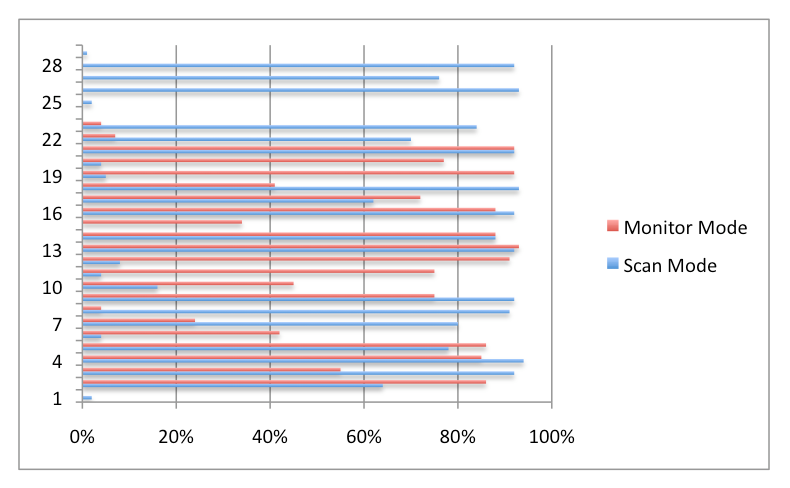
\includegraphics[scale=0.5]{cpu}}
\caption{The CPU usage comparison of Monitor and Scan mode}
\label{fig:cpu}
\end{figure}
Similar to our CPU usage results, the memory usage data was also disappointing. As shown in Figure~\ref{fig:memory}, the memory usage in monitor mode is even higher than scan mode initially. We think this is due in part to the fact that in monitor mode we have to perform an initial complete scan before we can switch over to the low overhead scan mode.  This, combined with the fact that monitor mode makes use of several more threads and an external JNI module seems to explain the difference.
\input{graph-memory}

In our tests of synchronization speed we finally got data that indicate that monitor version performs better. 
As we can see in Figure~\ref{fig:speed}, the speed of monitor mode is faster than scan mode on the client side. However, the 
server didn't show significant differences. This may be due to our current server side script using a pull-sync instead of push-sync as client side.

\begin{center}
  \begin{tabular}{ | l || c | c | c | c | }
    \hline
Speed	&	Local $\Rightarrow$ Server &	Server $\Rightarrow$ Local &	Local $\Rightarrow$ Server & Server $\Rightarrow$ Local\\
     	& (Scan Mode) &	(Scan Mode) &	(Monitor Mode)	& (Monitor Mode)\\
\hline\hline
Round 1	& 42.7 & 45.2 & 27.2 & 43.3 \\ \hline
Round 2	& 40.9 & 41.4 & 30.7 & 44.2 \\ \hline
Round 3	& 42.2 & 41	& 29.1 & 42.3	\\ \hline
Averge 	& 41.9 & 42.5 &	29 & 43.3 \\ 
	\hline
  \end{tabular}
\end{center}
 
\begin{figure}[htp]
\centering
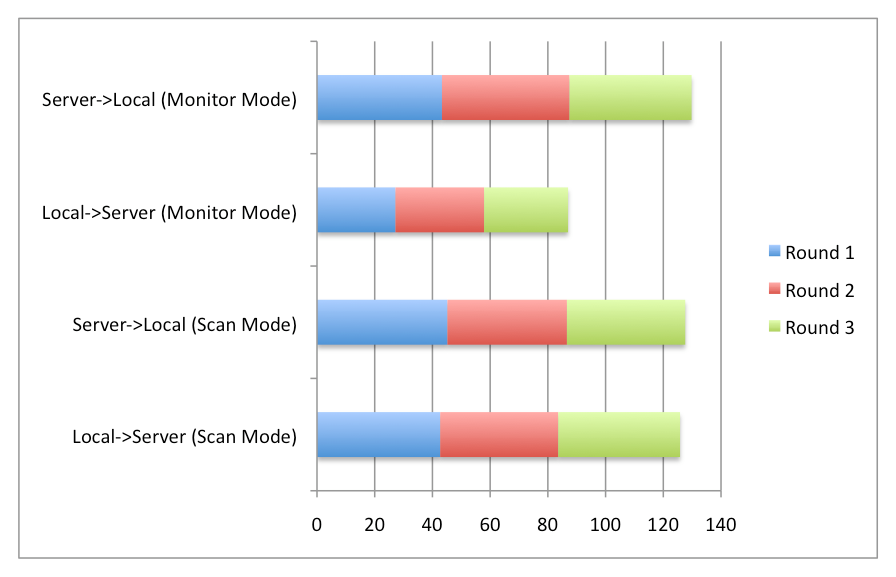
\includegraphics[scale=0.5]{speed}
\caption{Comparison of Synchronization Speed}\label{fig:speed}
\end{figure}
\section{Related Work}
\label{sec:Related}
There have been massive research on mobile device synchronization with different purpose. In our \teledroid\ project, 
we set up our goal to provide a mobile environment to access the cloud computing elements anywhere and anytime. We have 
looked into some other researches which have different goals but related with our project.

There's a research aimed at managing multiple devices in mobile information work~\cite{Oulasvirta:2007p1727}, which 
also need to satisfy the need of information synchronization. Some researches focus on the collaborative backup 
service~\cite{Courtes:2006p1734}, which have the problem of synchronization between different client when the backup 
copy is shared among multiple active client. We also noticed there is a hybrid approach to optimistic file system 
directory tree synchronization~\cite{Lindholm:2005p1760}. which mixed the two main approaches to optimistic file system 
synchronization: distributed file systems and file synchronizers. Also, we find a synchronization framework for personal mobile servers~\cite{Sinitsyn:2004p1738}, the high-level object-based storage API defined in this 
project is very much enlightening. We may as well provide APIs to allow other applications to control the \teledroid\ service.

However, in our primitive implementation, we choose to use the simplest way.
\section{Conclusions and Future Work}
\label{sec:Conclusions and Future Work}

While our experimental results weren't what we hoped, we're nevertheless optimistic about our approach.  Due to the complexity of the system and our limited time, we had comparatively few iterations of testing.  With this information in hand and with careful tracing we should expect to significantly reduce memory and cpu usage for the monitoring approach.  Our experiments were also more artificial than we would like.  Ideally we'd like to capture several real world scenarios.  Intuitively we would expect that real-world tests would feature longer times with no changes, and only short bursts where synchronization is needed.  Real world use might also have larger, more complicated directory trees with more files, which we would expect would favor a monitor-based system.

There are several factors that we didn't have time to implement and experiment with as well.  The period between communicating with the server could lengthen over time as no changes are detected.  As this period gets longer, at some point it may make sense to no longer maintain a constant connection with the server, only reconnecting when the period is up.  

On the other hand, if we keep the connection open and use a push based system from the server we wouldn't need to have an explicit waiting period at all.  This would require the Wifi radio to be actively listening however, which might raise the device's idle energy usage too high.

In short, we still believe that wireless synchronization may be feasible.  There are still a number of parameters that can be varied to get better performance before it's clear whether it is too inefficient.  We also remain convinced that as mobile devices become more capable, this feature will only become more desirable.


%\pagebreak

\small
\bibliographystyle{plain}
\bibliography{android}
\normalsize

\end{document}
